% ---
% Arquivo com os apêndices do Trabalho de Conclusão de Curso dos alunos
% Gabriel Takaoka Nishimura, Felippe Demarqui Ramos e Vivian Kimie Isuyama 
% da Escola Politécnica da Universidade de São Paulo
% ---
\chapter{Diagramas da Arquitetura}

\begin{figure}[h]
	\caption{\label{fig_sindrome_arq}Arquitetura do módulo de cálculo das síndromes.}
	\centering
	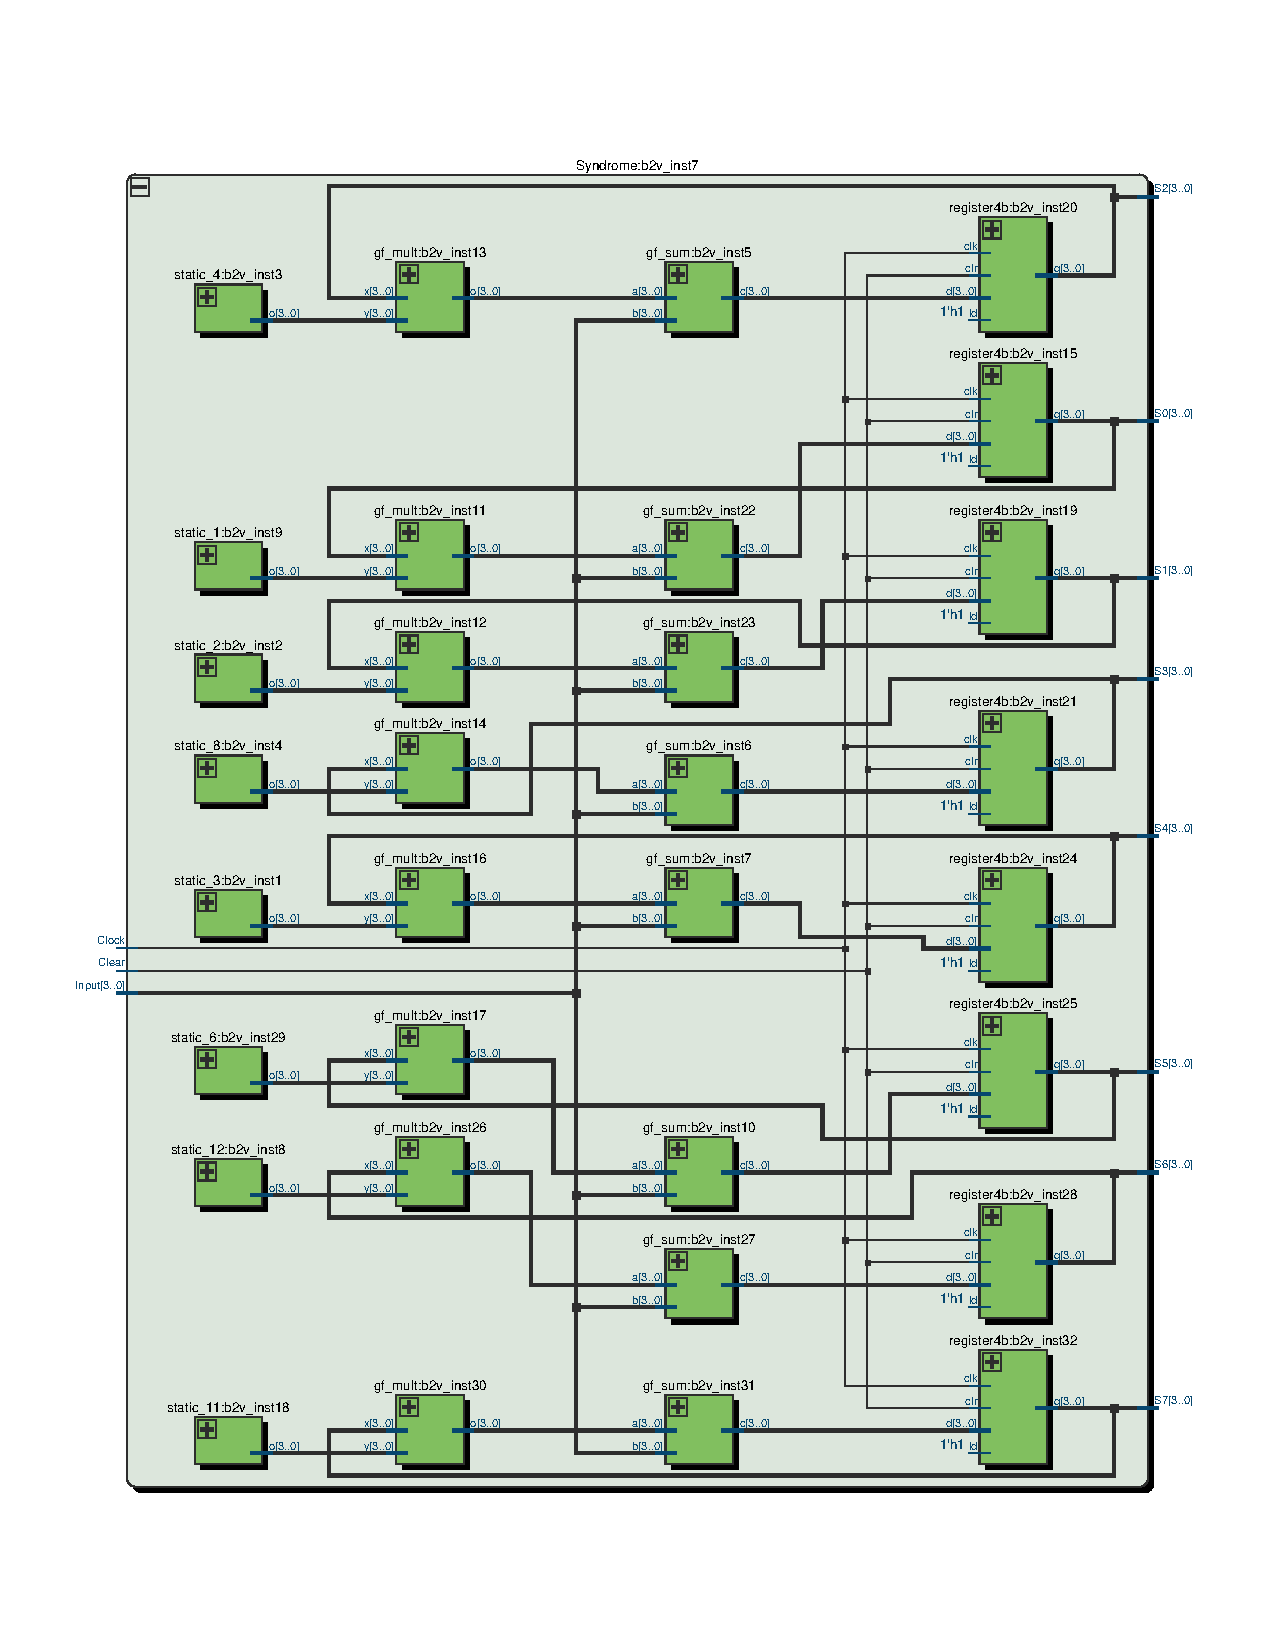
\includegraphics[width=0.5\textwidth, trim={0 1.2cm 0 3cm}, clip]{RS/SindromeRTL.pdf}
	\legend{Fonte: Autores.}
\end{figure}

\begin{figure}[h]
	\caption{\label{fig_berlekamp_arq}Arquitetura do módulo de Berlekamp-Massey.}
	\centering
	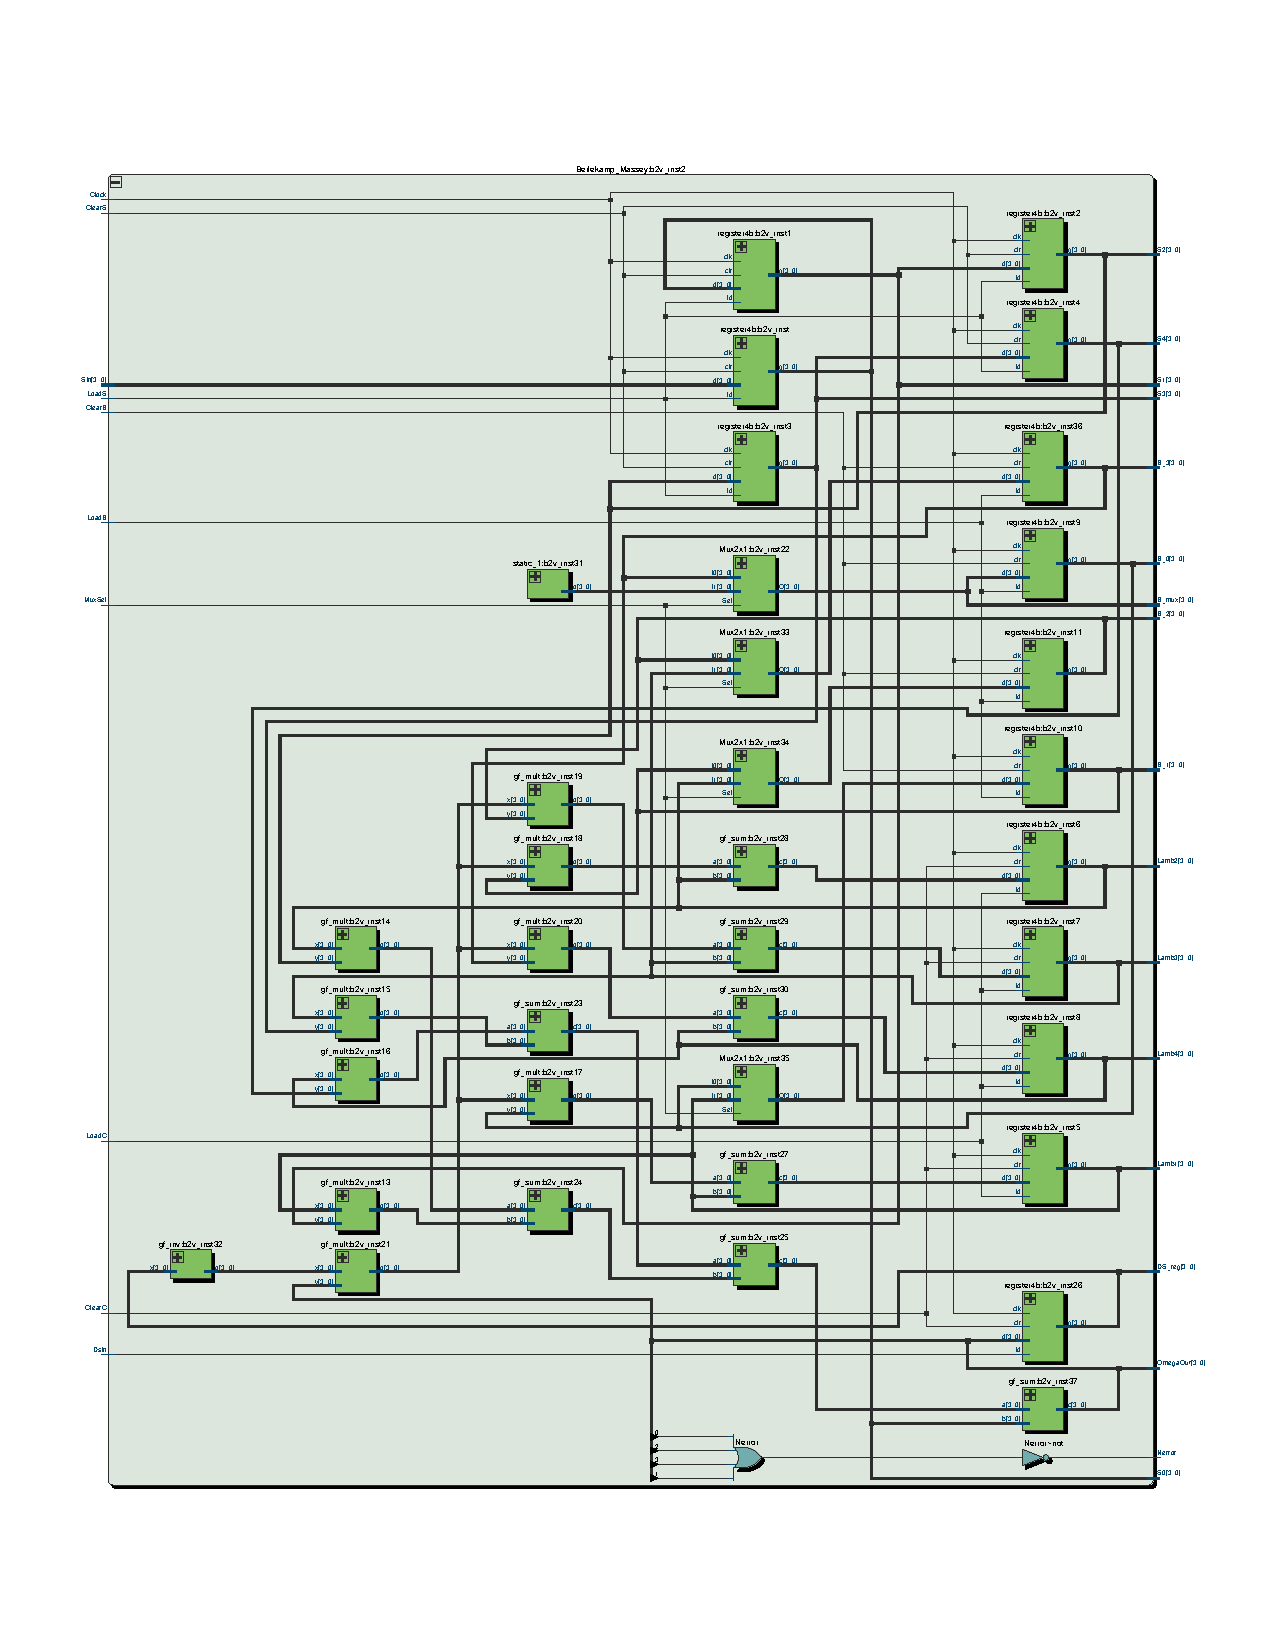
\includegraphics[width=0.5\textwidth, trim={0 1.2cm 0 3cm}, clip]{RS/BerlekampRTL.pdf}
	\legend{Fonte: Autores.}
\end{figure}

\begin{figure}[h]
	\caption{\label{fig_chienloc_arq}Arquitetura do módulo de busca de Chien: localização de erros.}
	\centering
	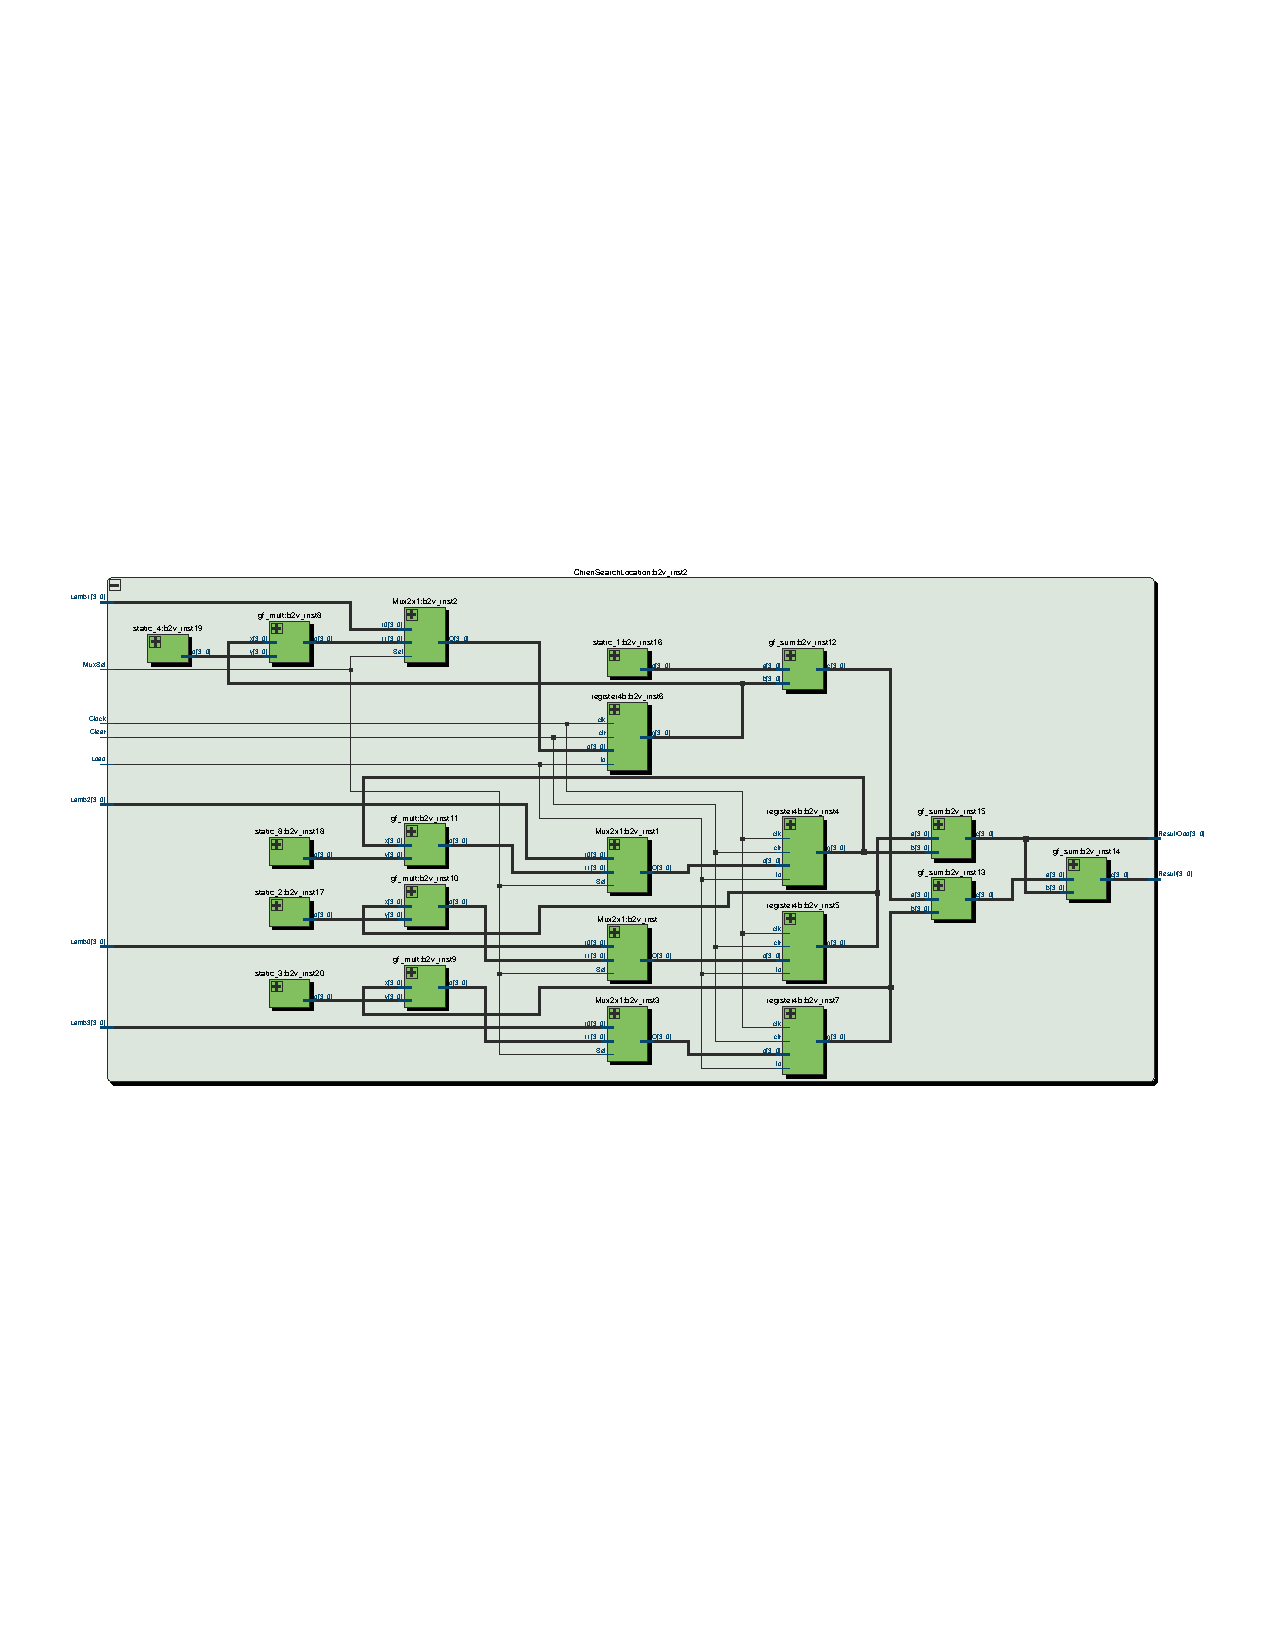
\includegraphics[width=0.5\textwidth, trim={0 8cm 0 9cm}, clip]{RS/ChienLocationRTL.pdf}
	\legend{Fonte: Autores.}
\end{figure}

\begin{figure}[h]
	\caption{\label{fig_chienval_arq}Arquitetura do módulo de busca de Chien: valores de erros.}
	\centering
	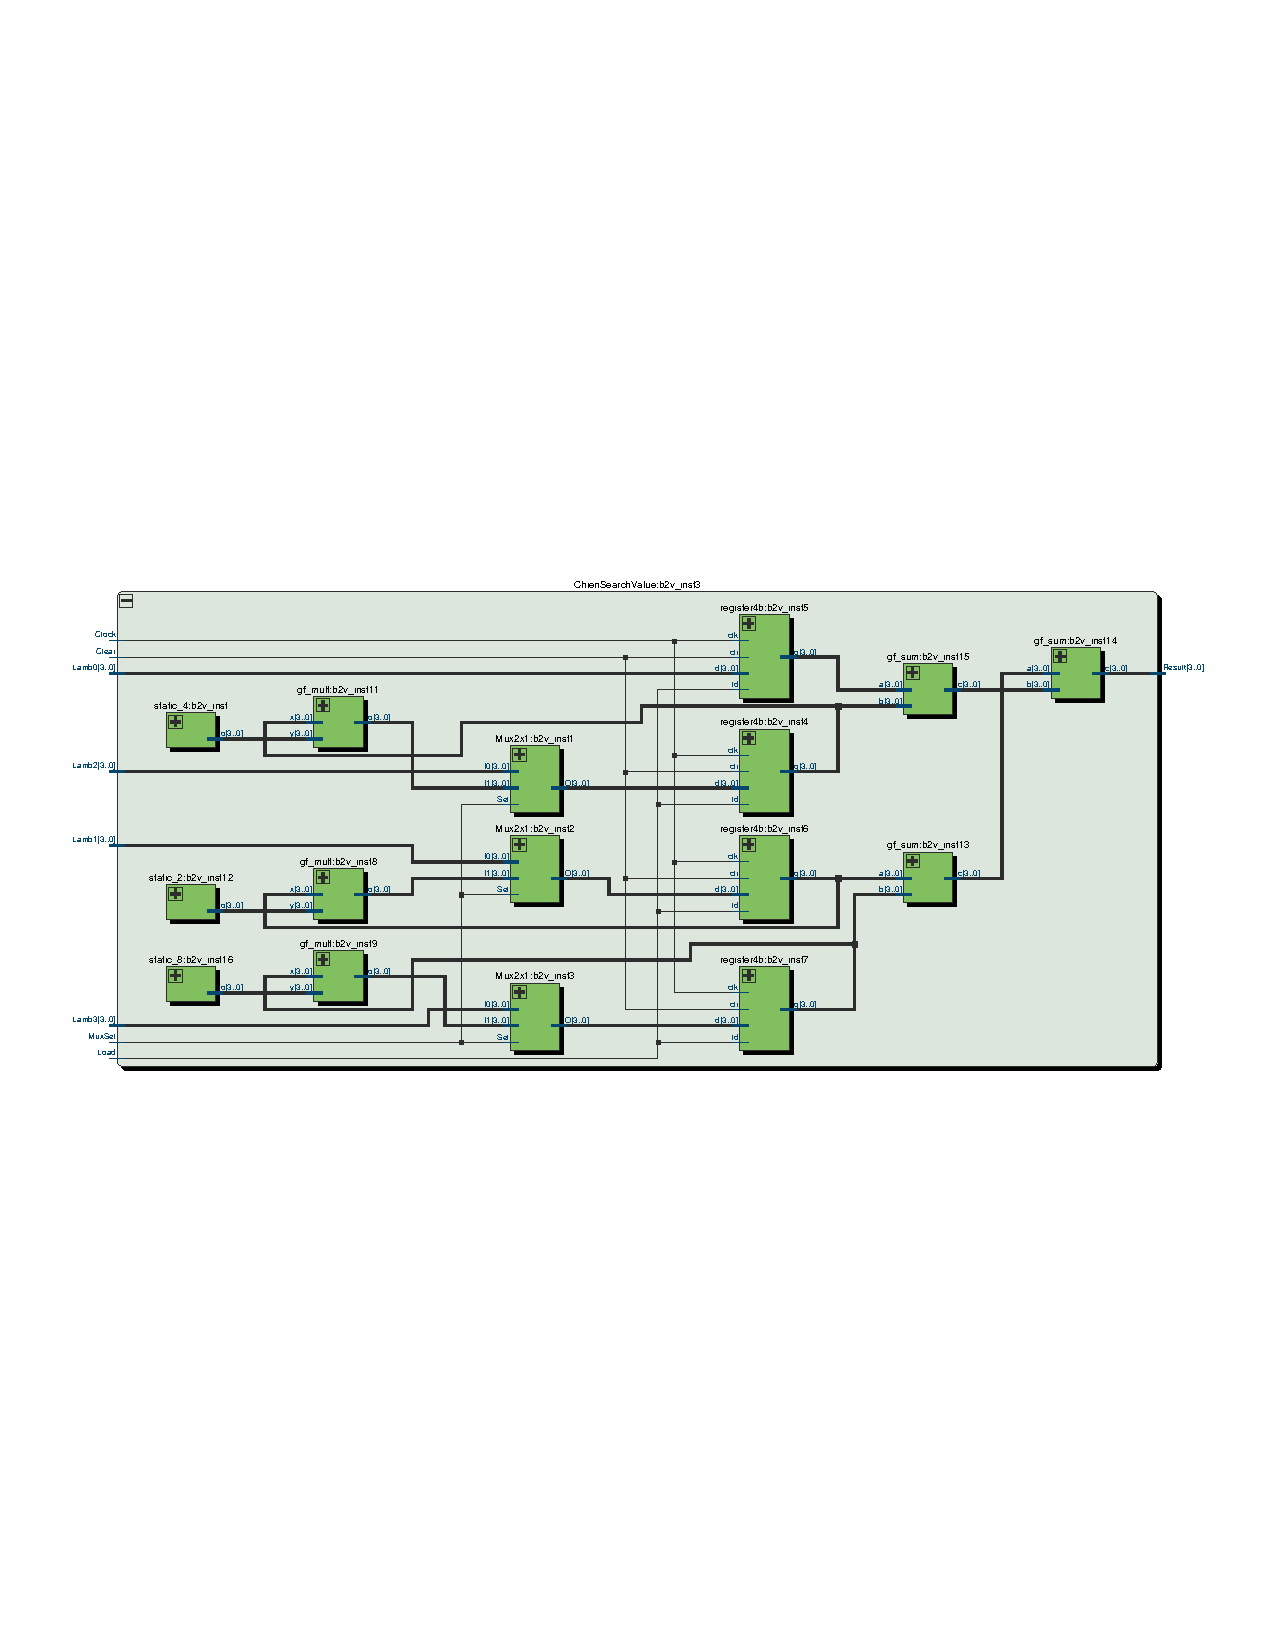
\includegraphics[width=0.5\textwidth, trim={0 8cm 0 9cm}, clip]{RS/ChienValueRTL.pdf}
	\legend{Fonte: Autores.}
\end{figure}

\begin{figure}[h]
	\caption{\label{figure:interleaver-rtl}Arquitetura do módulo de \textit{Interleaver}.}
	\centering
	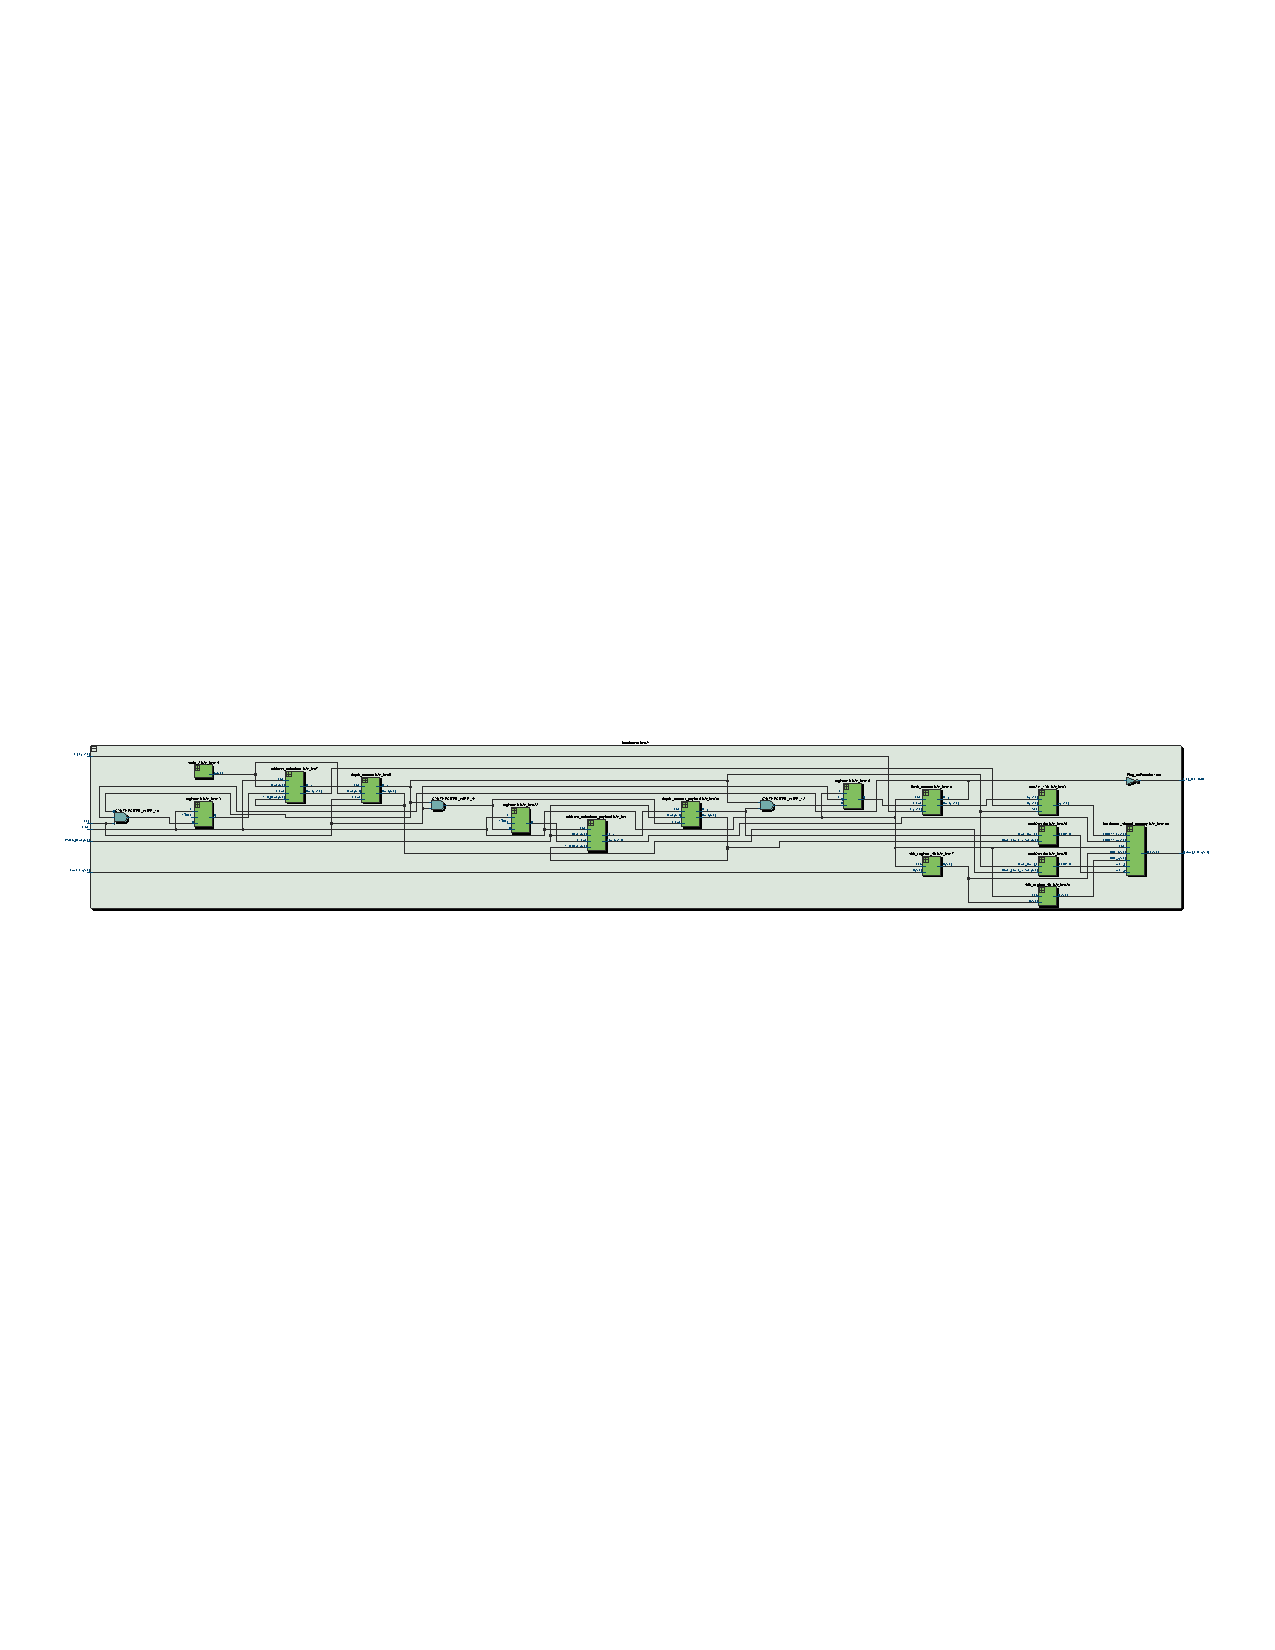
\includegraphics[width=1\textwidth, trim={0 12cm 0 12.5cm}, clip]{interleaver/rtl.pdf}
	\legend{Fonte: Autores.}
\end{figure}
\begin{figure}[h]
	\caption{\label{figure:sync-rtl}Arquitetura do módulo de Sincronização.}
	\centering
	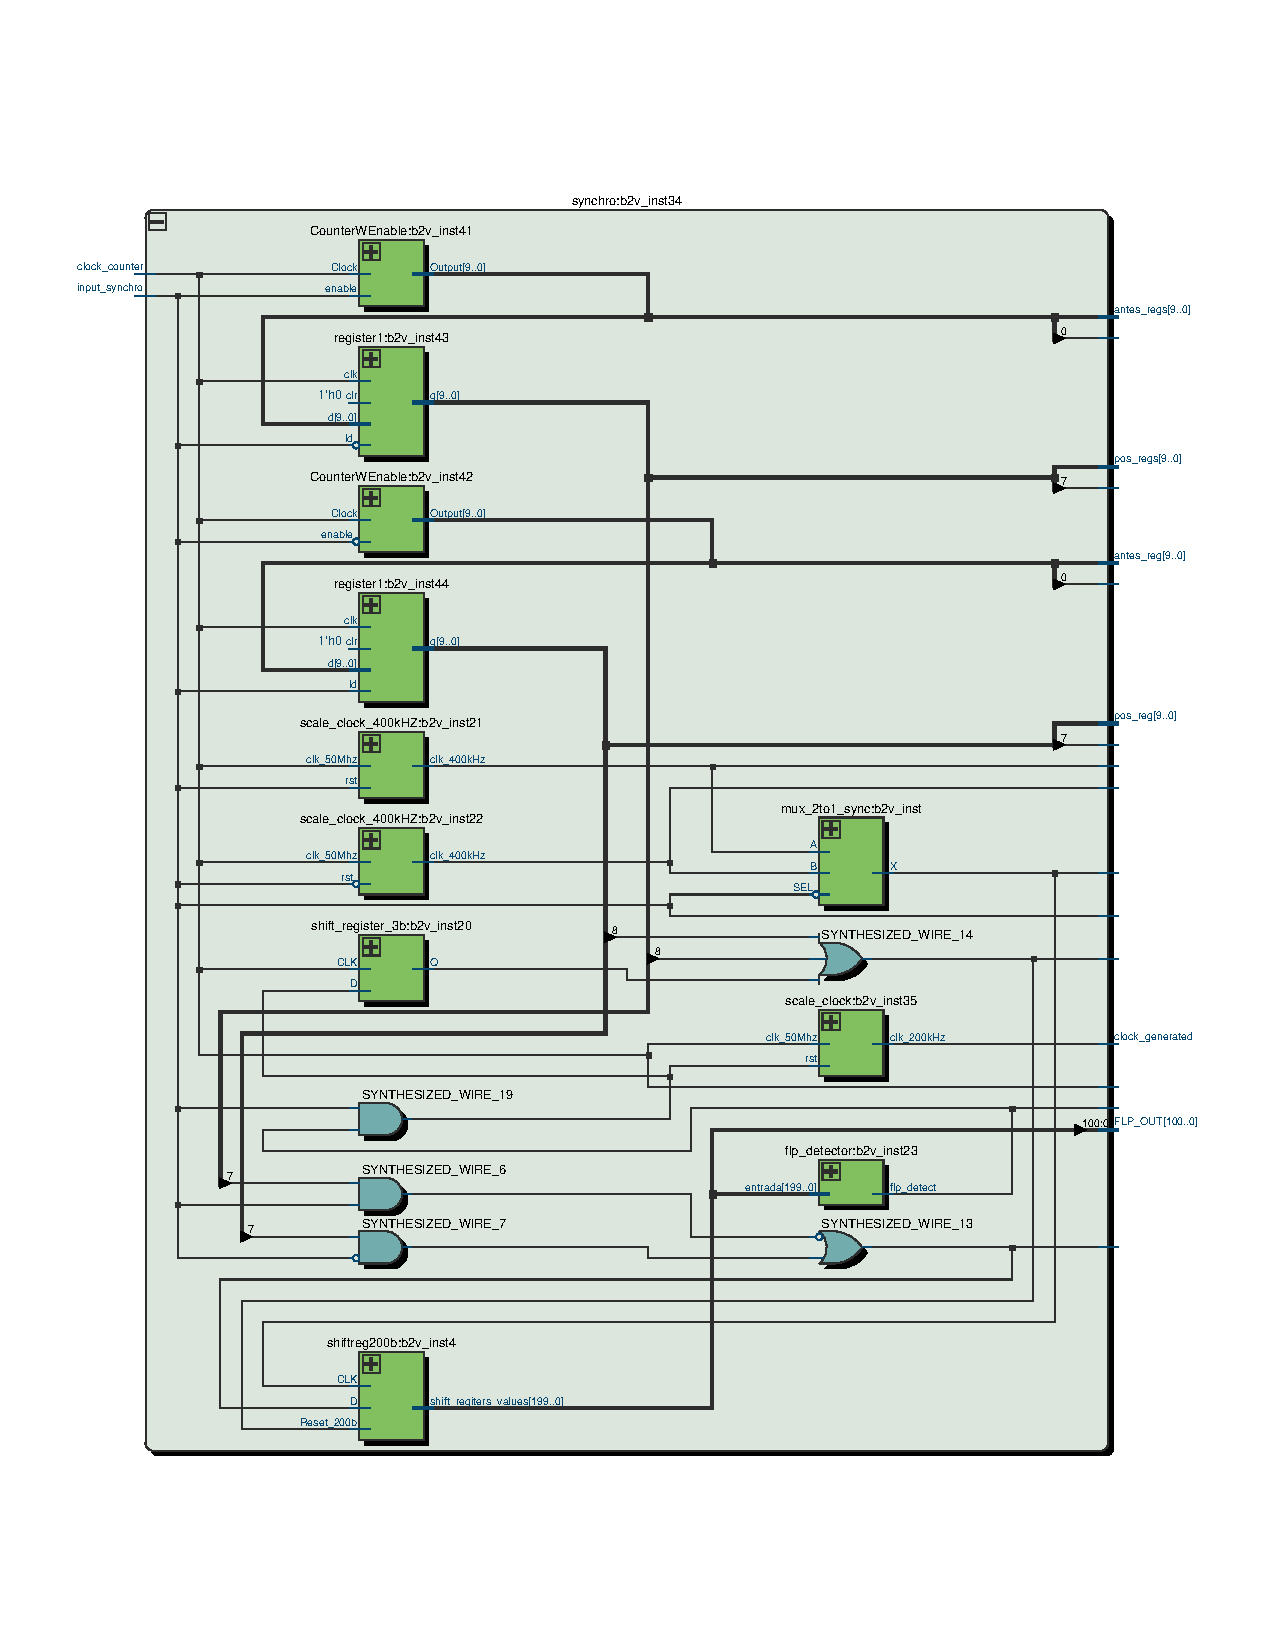
\includegraphics[width=0.5\textwidth, trim={0 2cm 0 3cm}, clip]{sync/rtl.pdf}
	\legend{Fonte: Autores.}
\end{figure}
\begin{figure}[h]
	\caption{\label{figure:manchester-decoder-rtl}Arquitetura do módulo de Decodificação Manchester.}
	\centering
	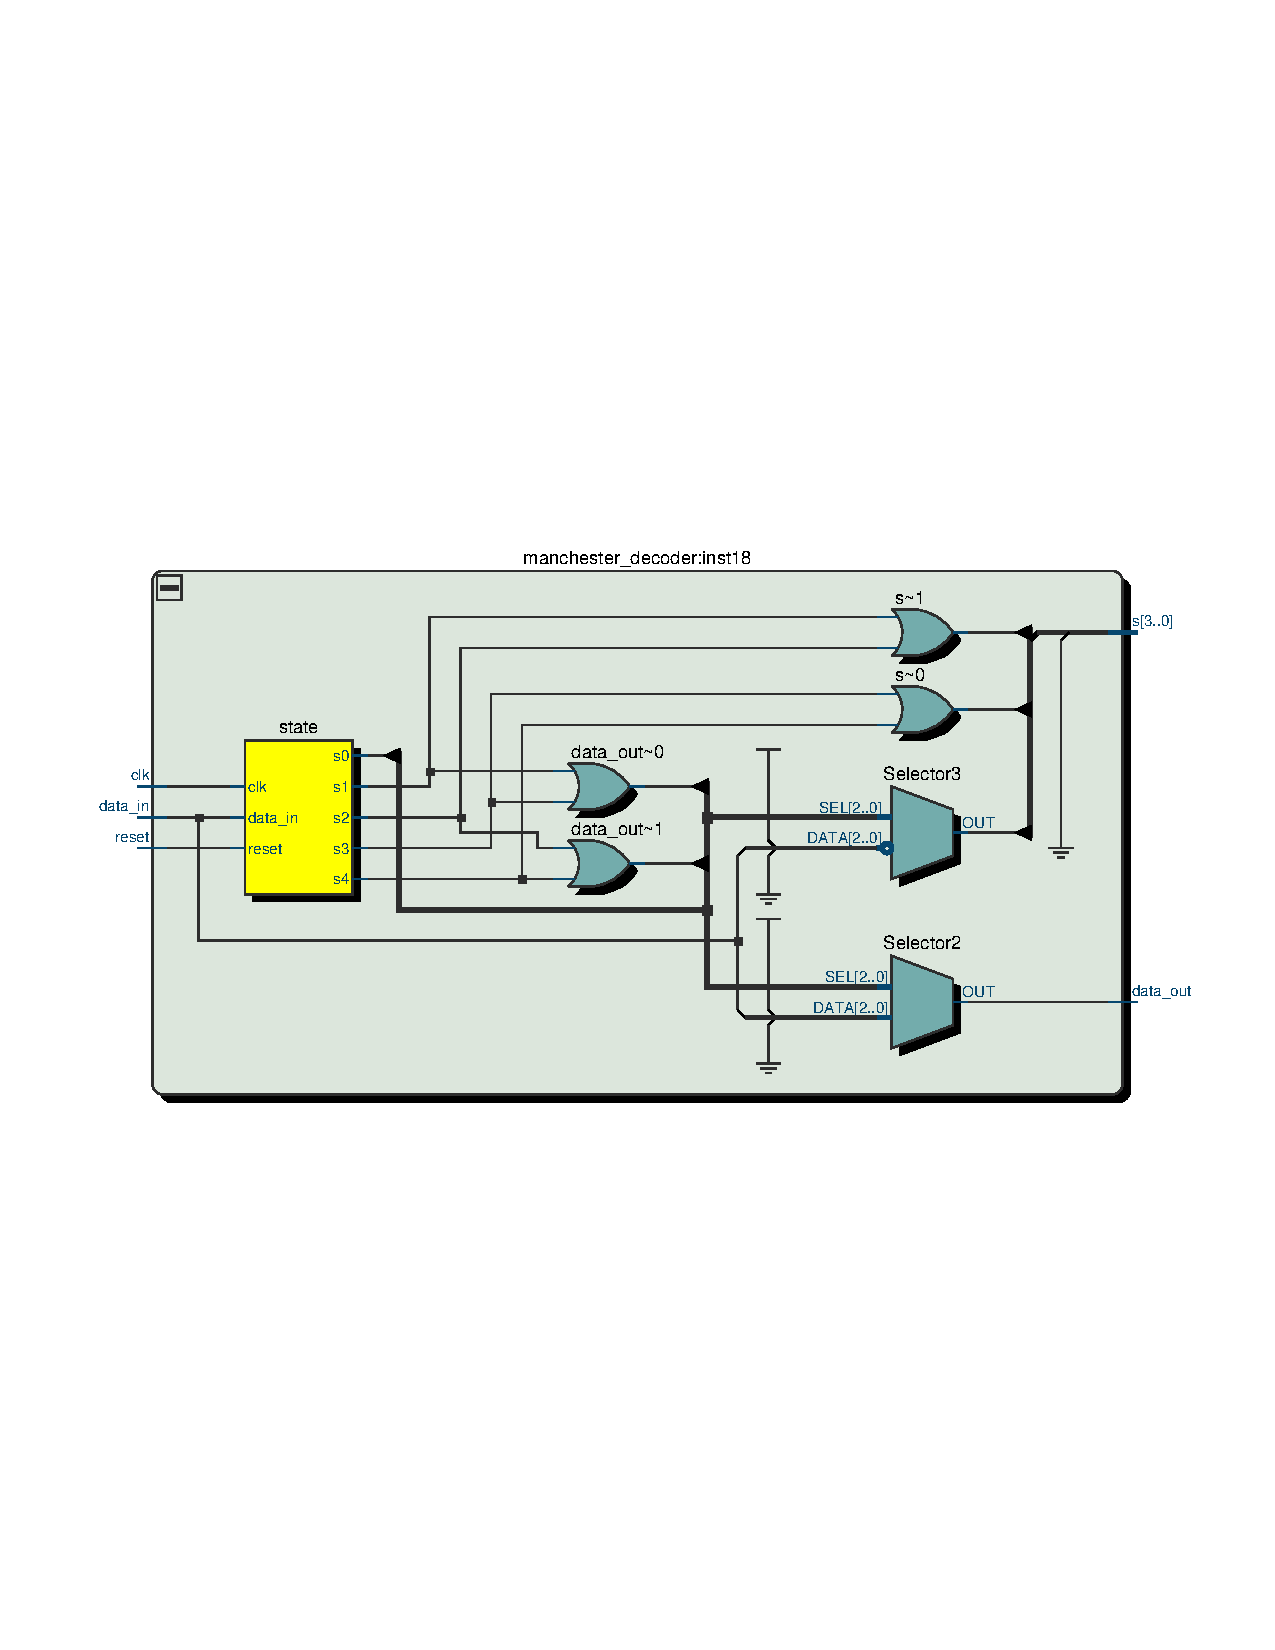
\includegraphics[width=0.5\textwidth, trim={0 7.7cm 0 8.5cm}, clip]{manchester/decoder-rtl.pdf}
	\legend{Fonte: Autores.}
\end{figure}

\begin{figure}[h]
	\caption{\label{figure:viterbi-rtl}Arquitetura do módulo de Decodificação Viterbi.}
	\centering
	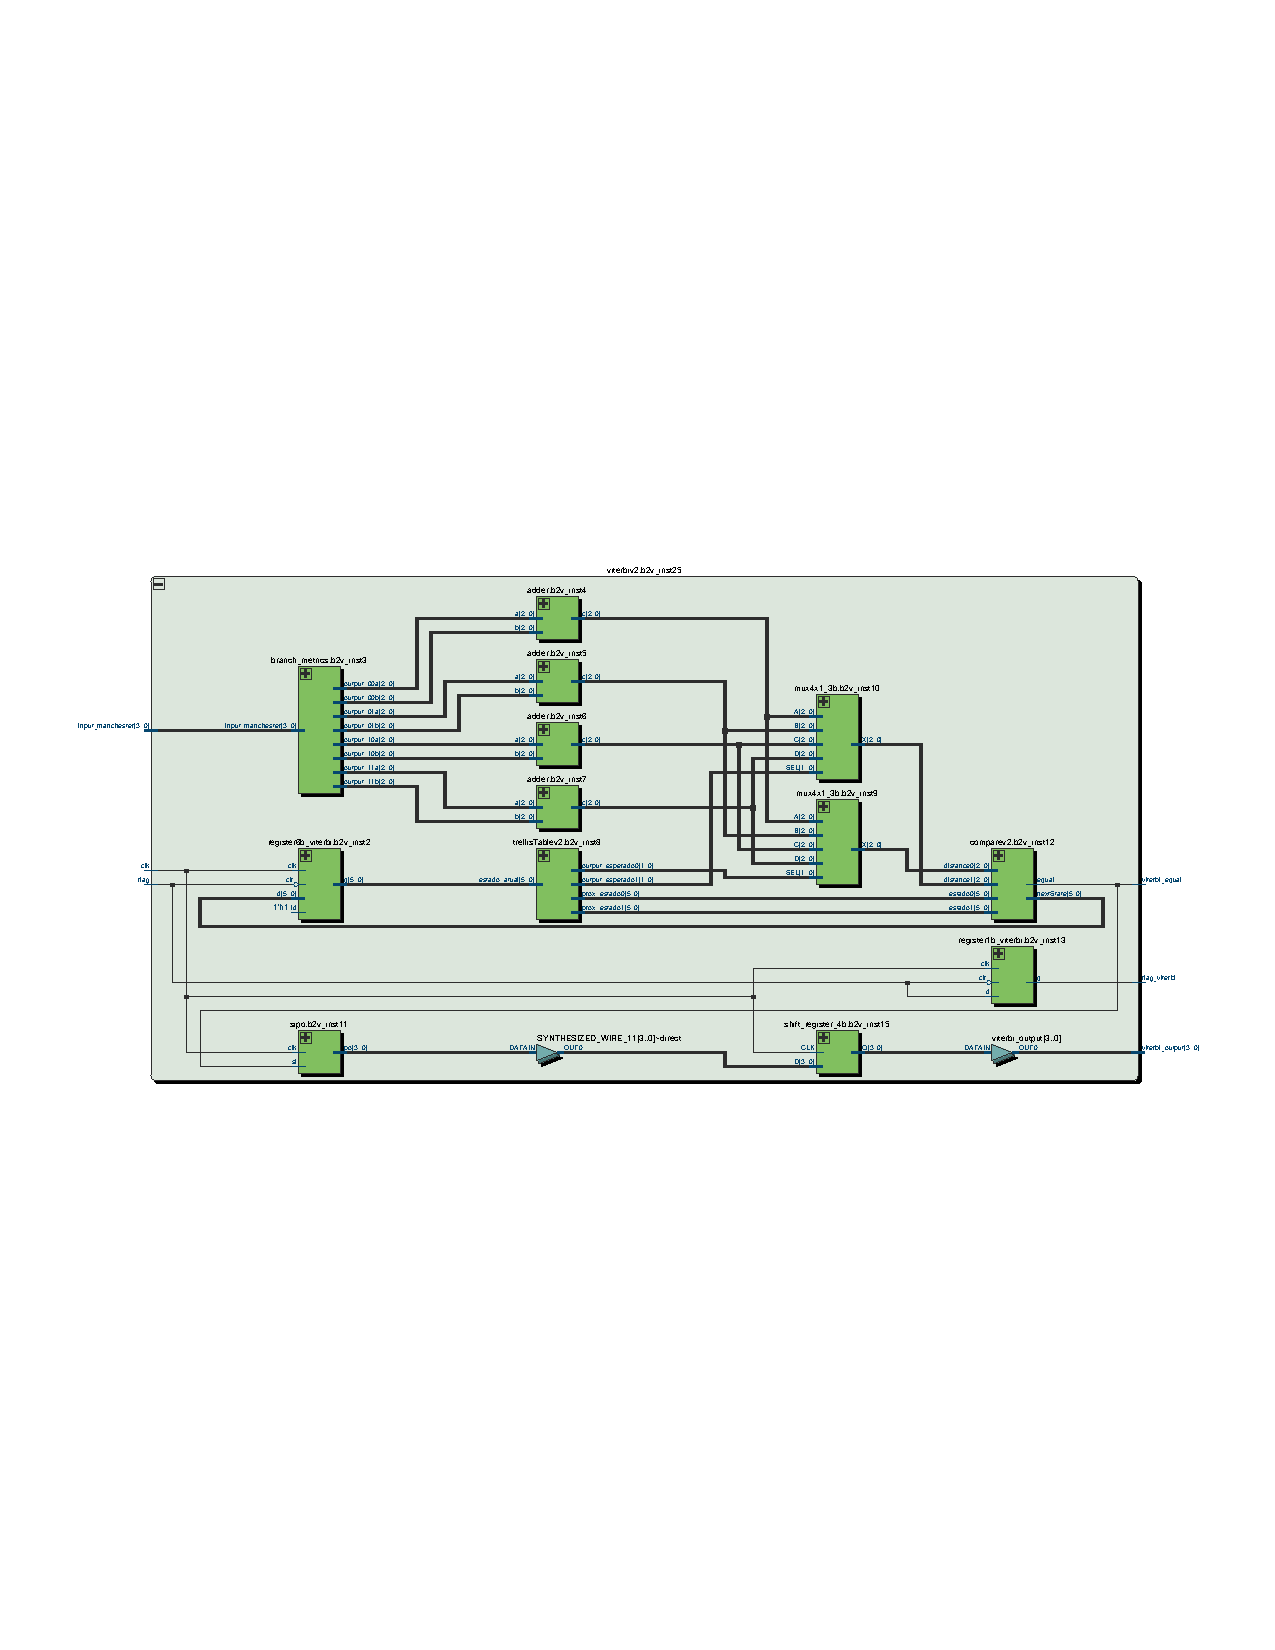
\includegraphics[width=0.5\textwidth, trim={0 7.7cm 0 8.5cm}, clip]{viterbi/rtl.pdf}
	\legend{Fonte: Autores.}
\end{figure}